\documentclass[12pt]{article}
\usepackage[total={18cm,22cm},top=3cm,left=2cm,right=2cm]{geometry}
\parindent=0mm
\usepackage[utf8]{inputenc}

\usepackage{hyperref}

\usepackage{multicol}

\usepackage{graphicx}

\usepackage{amsmath}

\usepackage{tikz}
\usepackage{enumitem}
\definecolor{azulF}{rgb}{.0,.0,.3}
\newcommand{\cnumero}[2]{\tikz[baseline=(myanchor.base)]
\node[minimum size=0.2cm,circle,
inner sep=1pt,draw, #2, thick, fill=#2](myanchor)
{\color{white}\bfseries\fontsize{8}{8}#1};}

\newcommand*{\itembolasazules}[1]{\protect\cnumero{#1}{azulF}}

\usepackage{fancyhdr}
\pagestyle{fancy}
\fancyhf{}
%TODO
\fancyhead[L]{TEORÍA DE SISTEMAS | GRUPO BETA | DIAGRAMA DE CONTEXTO}
%TODO
\fancyhead[R]{UNAH-VS}
\fancyfoot[C]{\thepage}

\renewcommand*\contentsname{Contenido}

\begin{document}
%*******************************************************
% Portada
%*******************************************************
\begin{titlepage}

  \begin{center}
    {\includegraphics[width=0.65\linewidth]{$HOME/Imágenes/Imgs/unahvs-logo.png}\par}
  
    {\bfseries\Huge Universidad Nacional Autónoma de\\
                     Honduras en el valle de Sula \par}
  
    \vspace{1cm}
  
%TODO
    {\scshape\huge TEORÍA DE SISTEMAS\par}
  
    \vspace{1cm}
  
%TODO
    {\scshape\Large 
      DIAGRAMA DE CONTEXTO 
    }
  
    \vfill 
    {\large Catedrático:\par} %TODO
    {\large Ing. Tania Melissa Pineda Godoy\par} %TODO
  
    \vfill
    {\large Grupo: \textbf{Beta} \par}

    \begin{tabular}{| l | c |}
      \hline
      Nombre & Numero de Cuenta\\ \hline
      Jonathan Asbel Sandoval Iscoa & 20192002289\\
      Carol Lizeth Lopez Garcia & 20152005774\\
      Maria Gaudalupe Aguilar Lopez & 20182030125\\
      Jimmy Xavier Triminio Hernandez & 20122008197 \\
      \hline
     \end{tabular}

    \vfill
    {\large FEBRERO 2023\par} %TODO

  \end{center}

\end{titlepage}

%*******************************************************
% Contenido 
%*******************************************************
\newpage
\tableofcontents

%*******************************************************
% Introducción
%*******************************************************
%\newpage
\section{Diagrama de Flujo de Datos de Contexto}
  Un diagrama de contexto, también conocido como un diagrama de de flujo de datos de contexto, es una representación gráfica de un proceso o sistema. Estos diagramas proporcionan una vista general del proceso y muestran los componentes principales del proceso. Estos componente incluyen entradas, salidas, almacenamiento de datos, procesamiento y flujos de datos. Estos diagramas se usan para identificar los componentes principales de un sistema y para documentar el flujo de datos en el sistema. El diagrama de contexto es el nivel mas alto en una jerarquía de diagramas de flujo de datos y suele ser el punto de partida para la creación de diagramas de flujo de datos de nivel superior.

\section{Ejercicio \#2}

Usted trabaja en la oficina del \textbf{cuartel general de la division de investigación de una delegación de policía} y esta desarrollando un sistema automatizado de rastreo de casos para la oficina del cuartel general para reemplazar el sistema manual actual.\\

Los casos son abiertos al publico cuando se recibe una forma de petición de investigación de otras decisiones en su delegación; ninguno de los casos se inicia internamente.\\

Se crea una carpeta nueva de caso, que contiene cualquier información de registro criminal basada en la verificación de diversas bases de datos de justicia criminal, y luego se manda a la oficina de investigación de campo apropiada.\\

Cuando el caso se completa, el cuartel general recibe un informe de investigación de la oficina de campo, el caso se cierra, y uan copia del reporte completo de investigación se envía a la oficina generadora.\\

Cada semana se manda a cada una de las oficinas del campo un listado que muestra los casos abiertos, completados y en marcha.\\

\begin{center}
  {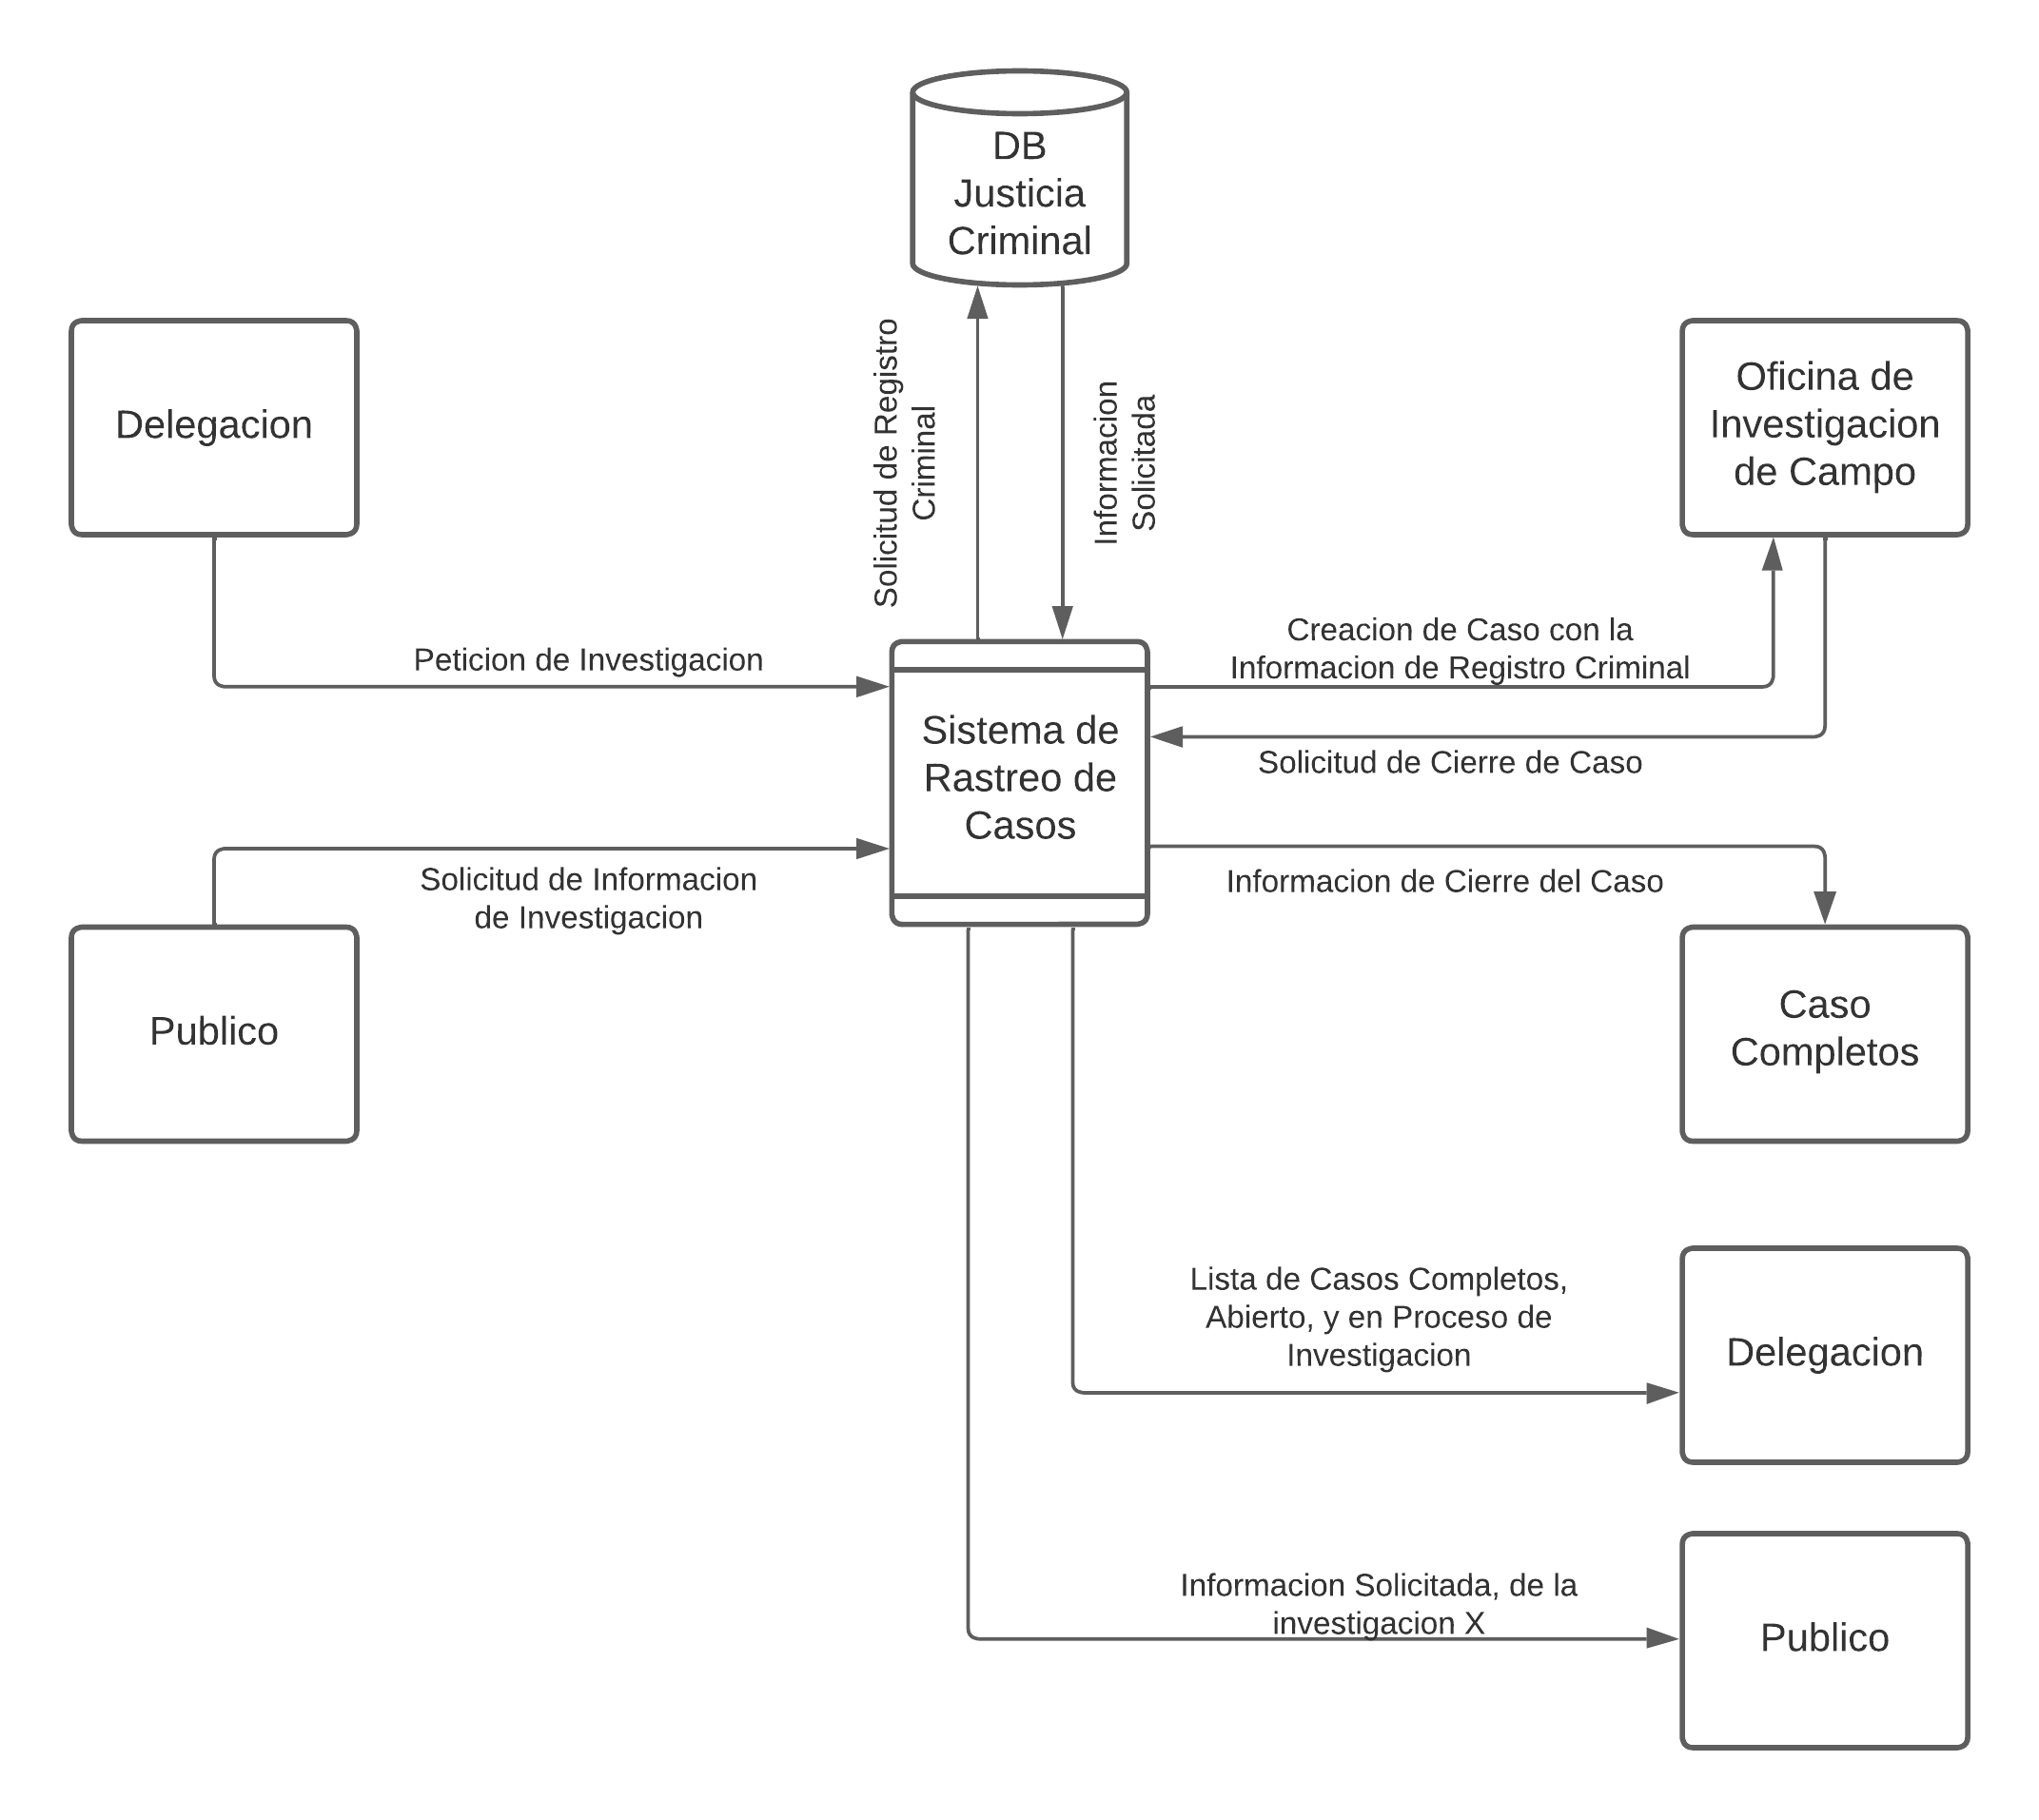
\includegraphics[width=0.65\linewidth]{imgs/Ejercicio2-DFD.png}\par}
\end{center}

\newpage
\section{Bibliografía}

\begin{enumerate}
   \item \textbf{Diagramas de Contexto}\\
        \href{https://es.venngage.com/blog/diagrama-de-contexto/}{venngage.com}

    \item \textbf{Diagramas de flujo de Datos}\\
        \href{https://miro.com/es/diagrama/que-es-diagrama-flujo-datos/}{miro.com}
\end{enumerate}


\end{document}

